\section{Pressure Regimes Are Not Universal Residency Thresholds}
\label{sec:pressure-regimes}

\begin{figure}[t]
    \centering
    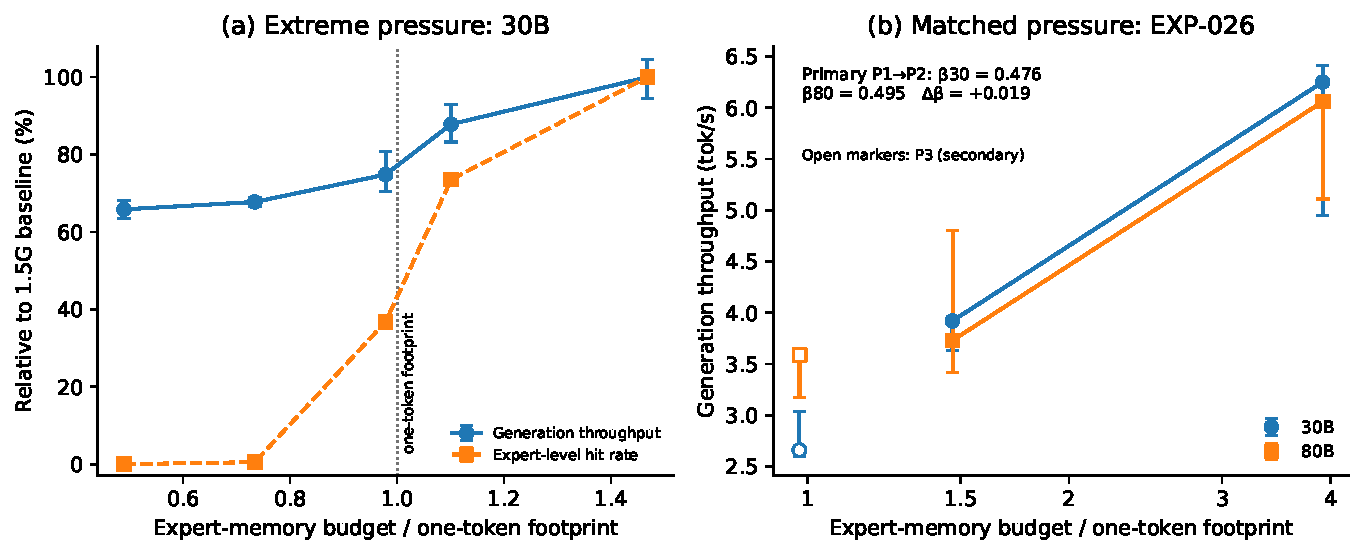
\includegraphics[width=\linewidth]{../experiments/EXP-026-30b-vs-80b-regimes/figures/cross_regime_synthesis.pdf}
    \caption{Reuse transitions and performance regimes are not universal residency thresholds. Panel (a) shows the 30B extreme-pressure result normalized to the 1.5\,GiB baseline: expert-level reuse collapses substantially faster than generation throughput, and execution continues below the one-token expert footprint. Panel (b) shows the matched-pressure comparison: the preregistered P1$\rightarrow$P2 pressure-response exponents are $\beta_{30}=0.476$ and $\beta_{80}=0.495$ ($\Delta\beta=+0.019$), so the models are not distinguished by the primary explanandum. Open markers show the secondary P3 condition.}
    \label{fig:pressure-regimes}
\end{figure}

The preceding sections show that cache capacity, hit rate, and layer allocation each capture only part of the system. We next ask whether a simple normalized capacity scale can nevertheless define a universal operating regime. Two experiments answer different parts of that question: EXP-022 pushes one model through extreme pressure, while EXP-026 compares both models at matched $M/F$ on the current runtime.

\subsection{Reuse can collapse before execution does}

Table~\ref{tab:extreme-pressure} summarizes the 30B primary arm of EXP-022. All 15 untraced performance launches and all 10 diagnostic launches completed validly down to 512\,MiB.

\begin{table}[t]
    \centering
    \caption{30B extreme-pressure means. The hit rate is the diagnostic workload gate-slice expert-level rate; throughput comes from separate untraced performance launches.}
    \label{tab:extreme-pressure}
    \small
    \begin{tabular}{lrrr}
        \toprule
        Budget & $M/F$ & Throughput (tok/s) & Expert-level hit (\%) \\
        \midrule
        1.5G  & 1.468 & 4.00 & 44.01 \\
        1152M & 1.101 & 3.51 & 32.37 \\
        1024M & 0.979 & 2.99 & 16.19 \\
        768M  & 0.734 & 2.71 & 0.232 \\
        512M  & 0.489 & 2.63 & 0.000 \\
        \bottomrule
    \end{tabular}
\end{table}

The two response variables separate sharply below the footprint. At $M/F=0.489$, the diagnostic expert-level hit rate has fallen to zero, yet throughput remains 2.63\,tok/s, approximately 65.8\% of the 1.5\,GiB baseline. At 768\,MiB ($0.734F$), reuse is already only 0.232\% while throughput remains 2.71\,tok/s.

Thus the one-token footprint marks neither a hard completion boundary nor a point at which useful throughput vanishes. It is more consistent with a transition scale for recency-based reuse under this workload. The preregistered historical H-5 falsifier at 30B/768\,MiB required an expert-level hit rate above 30\%; the observed mean was 0.2322\%. The historical prediction was therefore \emph{not falsified by this test}, but the experiment remains formally inconclusive because no positive support threshold had been specified.

The exploratory 80B arm reinforces the separation between low reuse and hard infeasibility. At 512\,MiB, two performance replicas completed in a degraded state while one encountered \nolinkurl{STORE_RESIDENCY_ABORT}. The mixed outcome does not establish 512\,MiB as an intrinsic physical lower bound for the model.

\begin{proposition}[The one-token footprint is not a hard execution threshold in the 30B extreme-pressure workload]
\label{prop:not-hard-threshold}
For the evaluated 30B runtime and workload, valid generation continues at expert-memory budgets strictly below the one-token footprint $F$.
\end{proposition}

\begin{proof}
The 30B footprint is approximately 1.0217\,GiB. Valid performance launches complete at both 768\,MiB ($0.734F$) and 512\,MiB ($0.489F$), with mean throughputs of 2.71 and 2.63\,tok/s. Therefore $M=F$ is not a necessary condition for execution in this workload.
\end{proof}

\subsection{The historical cross-model regime difference does not reproduce at matched pressure}

Historical sessions had suggested different sublinear pressure-response slopes for the two models, but those comparisons covered different normalized pressure regions and earlier binaries. EXP-026 prospectively removes two major confounds: the primary points are matched by $M/F$, and both models are measured on the current runtime within one session. Both models keep four generation threads, the thread condition of the historical comparison.

For the primary P1$\rightarrow$P2 comparison, the observed median throughputs are:

\begin{table}[t]
    \centering
    \caption{EXP-026 primary matched-pressure performance. Parentheses give the observed range over three valid launches.}
    \label{tab:exp026-primary}
    \small
    \begin{tabular}{lrr}
        \toprule
        & P1 & P2 \\
        \midrule
        30B & 6.25\ (4.95--6.41) & 3.92\ (3.63--3.96) \\
        80B & 6.06\ (5.11--6.06) & 3.73\ (3.42--4.80) \\
        \bottomrule
    \end{tabular}
\end{table}

The preregistered pressure-response exponents are
\begin{equation}
    \beta_{30}=0.4756076,
    \qquad
    \beta_{80}=0.4947870,
    \qquad
    \Delta\beta=+0.0191794 .
    \label{eq:exp026-beta}
\end{equation}
Their launch-pair envelopes are
\[
    \beta_{30}\in[0.2275,\,0.5797],
    \qquad
    \beta_{80}\in[0.0638,\,0.5833],
\]
which overlap strongly. Under the frozen decision rule, the primary explanandum is therefore \textbf{not distinguished}. The historical flatter-80B regime does not reproduce over the matched-$F$ P1--P2 region on the current runtime.

This is a non-reproduction, not a retrospective invalidation. The earlier regimes were measured over different $M/F$ regions on earlier binaries and remain valid descriptions of those sessions. The matched-pressure result is consistent with the possibility that normalization or pressure region contributed to the historical contrast, but it does not establish that either factor \emph{caused} it.

\subsection{Mechanism attribution remains inconclusive}

EXP-026 also collected traced diagnostic measurements intended to discriminate candidate explanations if the primary cross-model difference reproduced. Those diagnostic slopes do not agree with the untraced primary result:
\[
    \beta_{30,\mathrm{traced}}=0.4960,
    \qquad
    \beta_{80,\mathrm{traced}}=0.2266,
    \qquad
    \Delta\beta_{\mathrm{traced}}=-0.2694.
\]
The sign of the traced difference is opposite to the primary $\Delta\beta$, so the preregistered agreement gate fails. Consequently, the candidate mechanisms---routing concentration, slice-size/queue-depth effects, bookkeeping, and compute---are all \emph{not evaluable} against the primary explanandum. The EXP-026 lifecycle status is therefore INCONCLUSIVE even though the primary non-reproduction itself is informative.

The secondary P3 condition is reported descriptively in Figure~\ref{fig:pressure-regimes}. Its median throughput is 2.66\,tok/s for the 30B and 3.59\,tok/s for the 80B at $M/F\approx0.979$. This endpoint should not be used to replace the frozen P1$\rightarrow$P2 decision.

Taken together, EXP-022 and EXP-026 rule out a simple universal-threshold interpretation. Below $F$, reuse can collapse while execution continues; at matched pressure above $F$, the historical cross-model slope difference need not reproduce. Resident fraction and one-token footprint are useful coordinates, but neither is a complete performance law.
